\documentclass[twoside]{book}

% Packages required by doxygen
\usepackage{calc}
\usepackage{doxygen}
\usepackage{graphicx}
\usepackage[utf8]{inputenc}
\usepackage{makeidx}
\usepackage{multicol}
\usepackage{multirow}
\usepackage{textcomp}
\usepackage[table]{xcolor}

% Font selection
\usepackage[T1]{fontenc}
\usepackage{mathptmx}
\usepackage[scaled=.90]{helvet}
\usepackage{courier}
\usepackage{amssymb}
\usepackage{sectsty}
\renewcommand{\familydefault}{\sfdefault}
\allsectionsfont{%
  \fontseries{bc}\selectfont%
  \color{darkgray}%
}
\renewcommand{\DoxyLabelFont}{%
  \fontseries{bc}\selectfont%
  \color{darkgray}%
}

% Page & text layout
\usepackage{geometry}
\geometry{%
  a4paper,%
  top=2.5cm,%
  bottom=2.5cm,%
  left=2.5cm,%
  right=2.5cm%
}
\tolerance=750
\hfuzz=15pt
\hbadness=750
\setlength{\emergencystretch}{15pt}
\setlength{\parindent}{0cm}
\setlength{\parskip}{0.2cm}
\makeatletter
\renewcommand{\paragraph}{%
  \@startsection{paragraph}{4}{0ex}{-1.0ex}{1.0ex}{%
    \normalfont\normalsize\bfseries\SS@parafont%
  }%
}
\renewcommand{\subparagraph}{%
  \@startsection{subparagraph}{5}{0ex}{-1.0ex}{1.0ex}{%
    \normalfont\normalsize\bfseries\SS@subparafont%
  }%
}
\makeatother

% Headers & footers
\usepackage{fancyhdr}
\pagestyle{fancyplain}
\fancyhead[LE]{\fancyplain{}{\bfseries\thepage}}
\fancyhead[CE]{\fancyplain{}{}}
\fancyhead[RE]{\fancyplain{}{\bfseries\leftmark}}
\fancyhead[LO]{\fancyplain{}{\bfseries\rightmark}}
\fancyhead[CO]{\fancyplain{}{}}
\fancyhead[RO]{\fancyplain{}{\bfseries\thepage}}
\fancyfoot[LE]{\fancyplain{}{}}
\fancyfoot[CE]{\fancyplain{}{}}
\fancyfoot[RE]{\fancyplain{}{\bfseries\scriptsize Generated on Tue Feb 11 2014 16\-:38\-:30 for Chess by Doxygen }}
\fancyfoot[LO]{\fancyplain{}{\bfseries\scriptsize Generated on Tue Feb 11 2014 16\-:38\-:30 for Chess by Doxygen }}
\fancyfoot[CO]{\fancyplain{}{}}
\fancyfoot[RO]{\fancyplain{}{}}
\renewcommand{\footrulewidth}{0.4pt}
\renewcommand{\chaptermark}[1]{%
  \markboth{#1}{}%
}
\renewcommand{\sectionmark}[1]{%
  \markright{\thesection\ #1}%
}

% Indices & bibliography
\usepackage{natbib}
\usepackage[titles]{tocloft}
\setcounter{tocdepth}{3}
\setcounter{secnumdepth}{5}
\makeindex

% Hyperlinks (required, but should be loaded last)
\usepackage{ifpdf}
\ifpdf
  \usepackage[pdftex,pagebackref=true]{hyperref}
\else
  \usepackage[ps2pdf,pagebackref=true]{hyperref}
\fi
\hypersetup{%
  colorlinks=true,%
  linkcolor=blue,%
  citecolor=blue,%
  unicode%
}

% Custom commands
\newcommand{\clearemptydoublepage}{%
  \newpage{\pagestyle{empty}\cleardoublepage}%
}


%===== C O N T E N T S =====

\begin{document}

% Titlepage & ToC
\hypersetup{pageanchor=false}
\pagenumbering{roman}
\begin{titlepage}
\vspace*{7cm}
\begin{center}%
{\Large Chess \\[1ex]\large 1.\-1 }\\
\vspace*{1cm}
{\large Generated by Doxygen 1.8.6}\\
\vspace*{0.5cm}
{\small Tue Feb 11 2014 16:38:30}\\
\end{center}
\end{titlepage}
\clearemptydoublepage
\tableofcontents
\clearemptydoublepage
\pagenumbering{arabic}
\hypersetup{pageanchor=true}

%--- Begin generated contents ---
\chapter{Hierarchical Index}
\section{Class Hierarchy}
This inheritance list is sorted roughly, but not completely, alphabetically\-:\begin{DoxyCompactList}
\item \contentsline{section}{tests.\-All\-Tests}{\pageref{classtests_1_1_all_tests}}{}
\item \contentsline{section}{tests.\-Bishop\-Test}{\pageref{classtests_1_1_bishop_test}}{}
\item \contentsline{section}{tests.\-Board\-Test}{\pageref{classtests_1_1_board_test}}{}
\item \contentsline{section}{model.\-Chess}{\pageref{classmodel_1_1_chess}}{}
\item \contentsline{section}{view.\-Chess\-G\-U\-I}{\pageref{classview_1_1_chess_g_u_i}}{}
\item \contentsline{section}{tests.\-Chess\-Test}{\pageref{classtests_1_1_chess_test}}{}
\item Focus\-Listener\begin{DoxyCompactList}
\item \contentsline{section}{controller.\-Text\-Input}{\pageref{classcontroller_1_1_text_input}}{}
\end{DoxyCompactList}
\item \contentsline{section}{tests.\-King\-Test}{\pageref{classtests_1_1_king_test}}{}
\item \contentsline{section}{tests.\-Knight\-Test}{\pageref{classtests_1_1_knight_test}}{}
\item \contentsline{section}{tests.\-Pawn\-Test}{\pageref{classtests_1_1_pawn_test}}{}
\item \contentsline{section}{pieces.\-Piece}{\pageref{classpieces_1_1_piece}}{}
\begin{DoxyCompactList}
\item \contentsline{section}{pieces.\-Bishop}{\pageref{classpieces_1_1_bishop}}{}
\item \contentsline{section}{pieces.\-King}{\pageref{classpieces_1_1_king}}{}
\item \contentsline{section}{pieces.\-Knight}{\pageref{classpieces_1_1_knight}}{}
\item \contentsline{section}{pieces.\-Pawn}{\pageref{classpieces_1_1_pawn}}{}
\item \contentsline{section}{pieces.\-Queen}{\pageref{classpieces_1_1_queen}}{}
\item \contentsline{section}{pieces.\-Rock}{\pageref{classpieces_1_1_rock}}{}
\item \contentsline{section}{pieces.\-Rook}{\pageref{classpieces_1_1_rook}}{}
\item \contentsline{section}{pieces.\-Sentry}{\pageref{classpieces_1_1_sentry}}{}
\end{DoxyCompactList}
\item \contentsline{section}{tests.\-Piece\-Test}{\pageref{classtests_1_1_piece_test}}{}
\item \contentsline{section}{tests.\-Queen\-Test}{\pageref{classtests_1_1_queen_test}}{}
\item \contentsline{section}{tests.\-Rock\-Test}{\pageref{classtests_1_1_rock_test}}{}
\item \contentsline{section}{tests.\-Rook\-Test}{\pageref{classtests_1_1_rook_test}}{}
\item \contentsline{section}{tests.\-Sentry\-Test}{\pageref{classtests_1_1_sentry_test}}{}
\item \contentsline{section}{model.\-Space}{\pageref{classmodel_1_1_space}}{}
\item \contentsline{section}{controller.\-Spring\-Utilities}{\pageref{classcontroller_1_1_spring_utilities}}{}
\item \contentsline{section}{controller.\-User\-Input}{\pageref{classcontroller_1_1_user_input}}{}
\item \contentsline{section}{tests.\-User\-Input\-Test}{\pageref{classtests_1_1_user_input_test}}{}
\item Action\-Listener\begin{DoxyCompactList}
\item \contentsline{section}{controller.\-Text\-Input}{\pageref{classcontroller_1_1_text_input}}{}
\end{DoxyCompactList}
\item J\-Panel\begin{DoxyCompactList}
\item \contentsline{section}{controller.\-Text\-Input}{\pageref{classcontroller_1_1_text_input}}{}
\item \contentsline{section}{model.\-Board}{\pageref{classmodel_1_1_board}}{}
\end{DoxyCompactList}
\end{DoxyCompactList}

\chapter{Class Index}
\section{Class List}
Here are the classes, structs, unions and interfaces with brief descriptions\-:\begin{DoxyCompactList}
\item\contentsline{section}{\hyperlink{classtests_1_1_all_tests}{tests.\-All\-Tests} }{\pageref{classtests_1_1_all_tests}}{}
\item\contentsline{section}{\hyperlink{classpieces_1_1_bishop}{pieces.\-Bishop} }{\pageref{classpieces_1_1_bishop}}{}
\item\contentsline{section}{\hyperlink{classtests_1_1_bishop_test}{tests.\-Bishop\-Test} }{\pageref{classtests_1_1_bishop_test}}{}
\item\contentsline{section}{\hyperlink{classmodel_1_1_board}{model.\-Board} }{\pageref{classmodel_1_1_board}}{}
\item\contentsline{section}{\hyperlink{classtests_1_1_board_test}{tests.\-Board\-Test} }{\pageref{classtests_1_1_board_test}}{}
\item\contentsline{section}{\hyperlink{classmodel_1_1_chess}{model.\-Chess} }{\pageref{classmodel_1_1_chess}}{}
\item\contentsline{section}{\hyperlink{classview_1_1_chess_g_u_i}{view.\-Chess\-G\-U\-I} }{\pageref{classview_1_1_chess_g_u_i}}{}
\item\contentsline{section}{\hyperlink{classtests_1_1_chess_test}{tests.\-Chess\-Test} }{\pageref{classtests_1_1_chess_test}}{}
\item\contentsline{section}{\hyperlink{classpieces_1_1_king}{pieces.\-King} }{\pageref{classpieces_1_1_king}}{}
\item\contentsline{section}{\hyperlink{classtests_1_1_king_test}{tests.\-King\-Test} }{\pageref{classtests_1_1_king_test}}{}
\item\contentsline{section}{\hyperlink{classpieces_1_1_knight}{pieces.\-Knight} }{\pageref{classpieces_1_1_knight}}{}
\item\contentsline{section}{\hyperlink{classtests_1_1_knight_test}{tests.\-Knight\-Test} }{\pageref{classtests_1_1_knight_test}}{}
\item\contentsline{section}{\hyperlink{classpieces_1_1_pawn}{pieces.\-Pawn} }{\pageref{classpieces_1_1_pawn}}{}
\item\contentsline{section}{\hyperlink{classtests_1_1_pawn_test}{tests.\-Pawn\-Test} }{\pageref{classtests_1_1_pawn_test}}{}
\item\contentsline{section}{\hyperlink{classpieces_1_1_piece}{pieces.\-Piece} }{\pageref{classpieces_1_1_piece}}{}
\item\contentsline{section}{\hyperlink{classtests_1_1_piece_test}{tests.\-Piece\-Test} }{\pageref{classtests_1_1_piece_test}}{}
\item\contentsline{section}{\hyperlink{classpieces_1_1_queen}{pieces.\-Queen} }{\pageref{classpieces_1_1_queen}}{}
\item\contentsline{section}{\hyperlink{classtests_1_1_queen_test}{tests.\-Queen\-Test} }{\pageref{classtests_1_1_queen_test}}{}
\item\contentsline{section}{\hyperlink{classpieces_1_1_rock}{pieces.\-Rock} }{\pageref{classpieces_1_1_rock}}{}
\item\contentsline{section}{\hyperlink{classtests_1_1_rock_test}{tests.\-Rock\-Test} }{\pageref{classtests_1_1_rock_test}}{}
\item\contentsline{section}{\hyperlink{classpieces_1_1_rook}{pieces.\-Rook} }{\pageref{classpieces_1_1_rook}}{}
\item\contentsline{section}{\hyperlink{classtests_1_1_rook_test}{tests.\-Rook\-Test} }{\pageref{classtests_1_1_rook_test}}{}
\item\contentsline{section}{\hyperlink{classpieces_1_1_sentry}{pieces.\-Sentry} }{\pageref{classpieces_1_1_sentry}}{}
\item\contentsline{section}{\hyperlink{classtests_1_1_sentry_test}{tests.\-Sentry\-Test} }{\pageref{classtests_1_1_sentry_test}}{}
\item\contentsline{section}{\hyperlink{classmodel_1_1_space}{model.\-Space} }{\pageref{classmodel_1_1_space}}{}
\item\contentsline{section}{\hyperlink{classcontroller_1_1_spring_utilities}{controller.\-Spring\-Utilities} }{\pageref{classcontroller_1_1_spring_utilities}}{}
\item\contentsline{section}{\hyperlink{classcontroller_1_1_text_input}{controller.\-Text\-Input} }{\pageref{classcontroller_1_1_text_input}}{}
\item\contentsline{section}{\hyperlink{classcontroller_1_1_user_input}{controller.\-User\-Input} }{\pageref{classcontroller_1_1_user_input}}{}
\item\contentsline{section}{\hyperlink{classtests_1_1_user_input_test}{tests.\-User\-Input\-Test} }{\pageref{classtests_1_1_user_input_test}}{}
\end{DoxyCompactList}

\chapter{Class Documentation}
\hypertarget{class_bishop}{\section{Bishop Class Reference}
\label{class_bishop}\index{Bishop@{Bishop}}
}
Inheritance diagram for Bishop\-:\begin{figure}[H]
\begin{center}
\leavevmode
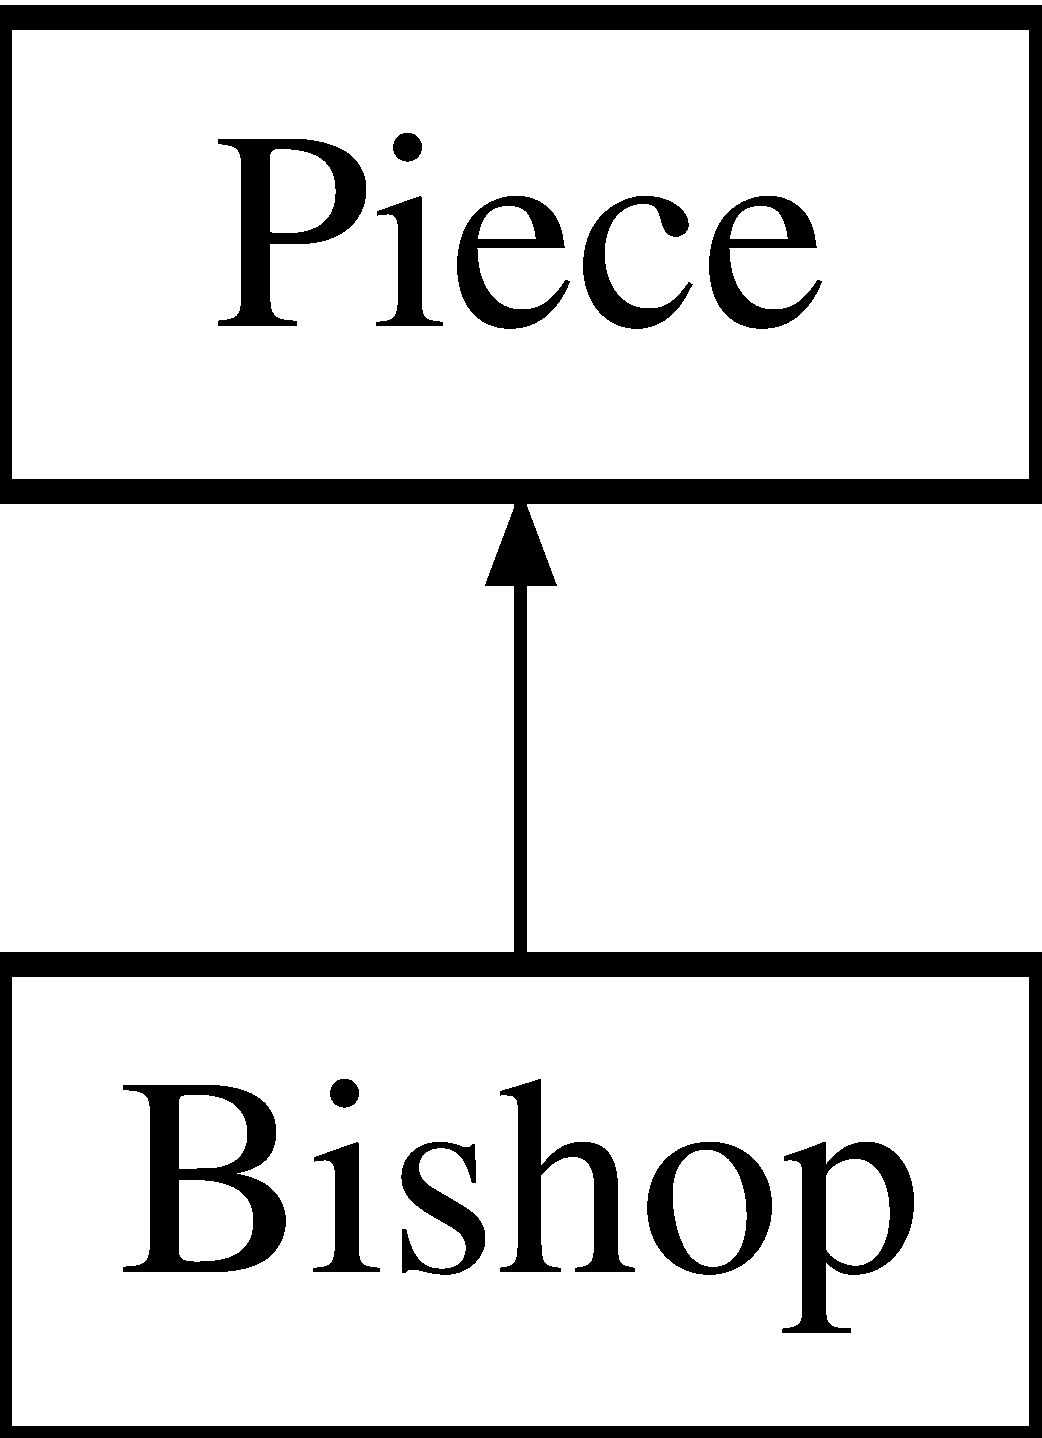
\includegraphics[height=2.000000cm]{class_bishop}
\end{center}
\end{figure}
\subsection*{Public Member Functions}
\begin{DoxyCompactItemize}
\item 
\hypertarget{class_bishop_acab26f3bb2c1de313918ada7efb8e0d3}{void {\bfseries update\-Moves} (\hyperlink{class_piece}{Piece}\mbox{[}$\,$\mbox{]}\mbox{[}$\,$\mbox{]} spaces, int rank, int file)}\label{class_bishop_acab26f3bb2c1de313918ada7efb8e0d3}

\end{DoxyCompactItemize}
\subsection*{Additional Inherited Members}


The documentation for this class was generated from the following file\-:\begin{DoxyCompactItemize}
\item 
src/Bishop.\-java\end{DoxyCompactItemize}

\hypertarget{class_board}{\section{Board Class Reference}
\label{class_board}\index{Board@{Board}}
}
\subsection*{Public Member Functions}
\begin{DoxyCompactItemize}
\item 
\hyperlink{class_board_aebf754535b8a0916d83200f22e18b7d2}{Board} (\hyperlink{class_board}{Board} other)
\item 
boolean \hyperlink{class_board_ae21b41dcb5ceec5c4e65b78cf1a7a4c2}{set\-Piece} (String piece, int rank, int file, Color player)
\item 
\hyperlink{class_piece}{Piece} \hyperlink{class_board_aea0f59c98263beace6443cd735d6805c}{get\-Piece} (int rank, int file)
\item 
boolean \hyperlink{class_board_ae0e4510755f6ae9d6ee19d583a11a33b}{move\-Piece} (int rstart, int fstart, int rtarget, int ftarget)
\item 
boolean \hyperlink{class_board_af4ea6b5281f049d33eec4833fa370765}{out\-Of\-Bounds} (int rank, int file)
\item 
void \hyperlink{class_board_a6a1cca4fd5509abd8ade2bb0c609bd20}{update\-Pieces} ()
\item 
boolean \hyperlink{class_board_a0b0b1d68cf48422fa95a14ce744c5ea2}{in\-Check} (Color player)
\item 
boolean \hyperlink{class_board_ab7e8e624384c4f17b31a931fbfb7e25d}{in\-Checkmate} (Color player)
\item 
boolean \hyperlink{class_board_a734bff11809a6e4b62c26456bffb966e}{in\-Stalemate} (Color player)
\end{DoxyCompactItemize}


\subsection{Constructor \& Destructor Documentation}
\hypertarget{class_board_aebf754535b8a0916d83200f22e18b7d2}{\index{Board@{Board}!Board@{Board}}
\index{Board@{Board}!Board@{Board}}
\subsubsection[{Board}]{\setlength{\rightskip}{0pt plus 5cm}Board.\-Board (
\begin{DoxyParamCaption}
\item[{{\bf Board}}]{other}
\end{DoxyParamCaption}
)}}\label{class_board_aebf754535b8a0916d83200f22e18b7d2}

\begin{DoxyParams}{Parameters}
{\em other} & \\
\hline
\end{DoxyParams}


\subsection{Member Function Documentation}
\hypertarget{class_board_aea0f59c98263beace6443cd735d6805c}{\index{Board@{Board}!get\-Piece@{get\-Piece}}
\index{get\-Piece@{get\-Piece}!Board@{Board}}
\subsubsection[{get\-Piece}]{\setlength{\rightskip}{0pt plus 5cm}{\bf Piece} Board.\-get\-Piece (
\begin{DoxyParamCaption}
\item[{int}]{rank, }
\item[{int}]{file}
\end{DoxyParamCaption}
)}}\label{class_board_aea0f59c98263beace6443cd735d6805c}

\begin{DoxyParams}{Parameters}
{\em rank} & \\
\hline
{\em file} & \\
\hline
\end{DoxyParams}
\begin{DoxyReturn}{Returns}
the piece at a given space 
\end{DoxyReturn}
\hypertarget{class_board_a0b0b1d68cf48422fa95a14ce744c5ea2}{\index{Board@{Board}!in\-Check@{in\-Check}}
\index{in\-Check@{in\-Check}!Board@{Board}}
\subsubsection[{in\-Check}]{\setlength{\rightskip}{0pt plus 5cm}boolean Board.\-in\-Check (
\begin{DoxyParamCaption}
\item[{Color}]{player}
\end{DoxyParamCaption}
)}}\label{class_board_a0b0b1d68cf48422fa95a14ce744c5ea2}
\begin{DoxyReturn}{Returns}

\end{DoxyReturn}
\hypertarget{class_board_ab7e8e624384c4f17b31a931fbfb7e25d}{\index{Board@{Board}!in\-Checkmate@{in\-Checkmate}}
\index{in\-Checkmate@{in\-Checkmate}!Board@{Board}}
\subsubsection[{in\-Checkmate}]{\setlength{\rightskip}{0pt plus 5cm}boolean Board.\-in\-Checkmate (
\begin{DoxyParamCaption}
\item[{Color}]{player}
\end{DoxyParamCaption}
)}}\label{class_board_ab7e8e624384c4f17b31a931fbfb7e25d}

\begin{DoxyParams}{Parameters}
{\em player} & \\
\hline
\end{DoxyParams}
\begin{DoxyReturn}{Returns}

\end{DoxyReturn}
\hypertarget{class_board_a734bff11809a6e4b62c26456bffb966e}{\index{Board@{Board}!in\-Stalemate@{in\-Stalemate}}
\index{in\-Stalemate@{in\-Stalemate}!Board@{Board}}
\subsubsection[{in\-Stalemate}]{\setlength{\rightskip}{0pt plus 5cm}boolean Board.\-in\-Stalemate (
\begin{DoxyParamCaption}
\item[{Color}]{player}
\end{DoxyParamCaption}
)}}\label{class_board_a734bff11809a6e4b62c26456bffb966e}

\begin{DoxyParams}{Parameters}
{\em player} & \\
\hline
\end{DoxyParams}
\begin{DoxyReturn}{Returns}

\end{DoxyReturn}
\hypertarget{class_board_ae0e4510755f6ae9d6ee19d583a11a33b}{\index{Board@{Board}!move\-Piece@{move\-Piece}}
\index{move\-Piece@{move\-Piece}!Board@{Board}}
\subsubsection[{move\-Piece}]{\setlength{\rightskip}{0pt plus 5cm}boolean Board.\-move\-Piece (
\begin{DoxyParamCaption}
\item[{int}]{rstart, }
\item[{int}]{fstart, }
\item[{int}]{rtarget, }
\item[{int}]{ftarget}
\end{DoxyParamCaption}
)}}\label{class_board_ae0e4510755f6ae9d6ee19d583a11a33b}

\begin{DoxyParams}{Parameters}
{\em rstart} & \\
\hline
{\em fstart} & \\
\hline
{\em rtarget} & \\
\hline
{\em ftarget} & \\
\hline
\end{DoxyParams}
\begin{DoxyReturn}{Returns}
true if the move was successful false otherwise 
\end{DoxyReturn}
\hypertarget{class_board_af4ea6b5281f049d33eec4833fa370765}{\index{Board@{Board}!out\-Of\-Bounds@{out\-Of\-Bounds}}
\index{out\-Of\-Bounds@{out\-Of\-Bounds}!Board@{Board}}
\subsubsection[{out\-Of\-Bounds}]{\setlength{\rightskip}{0pt plus 5cm}boolean Board.\-out\-Of\-Bounds (
\begin{DoxyParamCaption}
\item[{int}]{rank, }
\item[{int}]{file}
\end{DoxyParamCaption}
)}}\label{class_board_af4ea6b5281f049d33eec4833fa370765}

\begin{DoxyParams}{Parameters}
{\em rank} & \\
\hline
{\em file} & \\
\hline
\end{DoxyParams}
\begin{DoxyReturn}{Returns}
true if the position given is not a valid board position. 
\end{DoxyReturn}
\hypertarget{class_board_ae21b41dcb5ceec5c4e65b78cf1a7a4c2}{\index{Board@{Board}!set\-Piece@{set\-Piece}}
\index{set\-Piece@{set\-Piece}!Board@{Board}}
\subsubsection[{set\-Piece}]{\setlength{\rightskip}{0pt plus 5cm}boolean Board.\-set\-Piece (
\begin{DoxyParamCaption}
\item[{String}]{piece, }
\item[{int}]{rank, }
\item[{int}]{file, }
\item[{Color}]{player}
\end{DoxyParamCaption}
)}}\label{class_board_ae21b41dcb5ceec5c4e65b78cf1a7a4c2}

\begin{DoxyParams}{Parameters}
{\em piece} & \\
\hline
{\em rank} & \\
\hline
{\em file} & \\
\hline
{\em player} & \\
\hline
\end{DoxyParams}
\begin{DoxyReturn}{Returns}
true if the piece was set successfully 
\end{DoxyReturn}
\hypertarget{class_board_a6a1cca4fd5509abd8ade2bb0c609bd20}{\index{Board@{Board}!update\-Pieces@{update\-Pieces}}
\index{update\-Pieces@{update\-Pieces}!Board@{Board}}
\subsubsection[{update\-Pieces}]{\setlength{\rightskip}{0pt plus 5cm}void Board.\-update\-Pieces (
\begin{DoxyParamCaption}
{}
\end{DoxyParamCaption}
)}}\label{class_board_a6a1cca4fd5509abd8ade2bb0c609bd20}
We need to maintain possible moves for each piece to detect game-\/ending conditions. 

The documentation for this class was generated from the following file\-:\begin{DoxyCompactItemize}
\item 
src/Board.\-java\end{DoxyCompactItemize}

\hypertarget{class_chess}{\section{Chess Class Reference}
\label{class_chess}\index{Chess@{Chess}}
}
\subsection*{Static Public Attributes}
\begin{DoxyCompactItemize}
\item 
static final String\mbox{[}$\,$\mbox{]} {\bfseries init\-List}
\end{DoxyCompactItemize}


\subsection{Member Data Documentation}
\hypertarget{class_chess_a40e36ddfeea1126e7c4b9701d758d15b}{\index{Chess@{Chess}!init\-List@{init\-List}}
\index{init\-List@{init\-List}!Chess@{Chess}}
\subsubsection[{init\-List}]{\setlength{\rightskip}{0pt plus 5cm}final String \mbox{[}$\,$\mbox{]} Chess.\-init\-List\hspace{0.3cm}{\ttfamily [static]}}}\label{class_chess_a40e36ddfeea1126e7c4b9701d758d15b}
{\bfseries Initial value\-:}
\begin{DoxyCode}
= \{\textcolor{stringliteral}{"Rook"},\textcolor{stringliteral}{"Knight"},\textcolor{stringliteral}{"Bishop"},\textcolor{stringliteral}{"Queen"},
                                              \textcolor{stringliteral}{"King"},\textcolor{stringliteral}{"Bishop"},\textcolor{stringliteral}{"Knight"},\textcolor{stringliteral}{"Rook"}\}
\end{DoxyCode}


The documentation for this class was generated from the following file\-:\begin{DoxyCompactItemize}
\item 
src/Chess.\-java\end{DoxyCompactItemize}

\hypertarget{class_king}{\section{King Class Reference}
\label{class_king}\index{King@{King}}
}
Inheritance diagram for King\-:\begin{figure}[H]
\begin{center}
\leavevmode
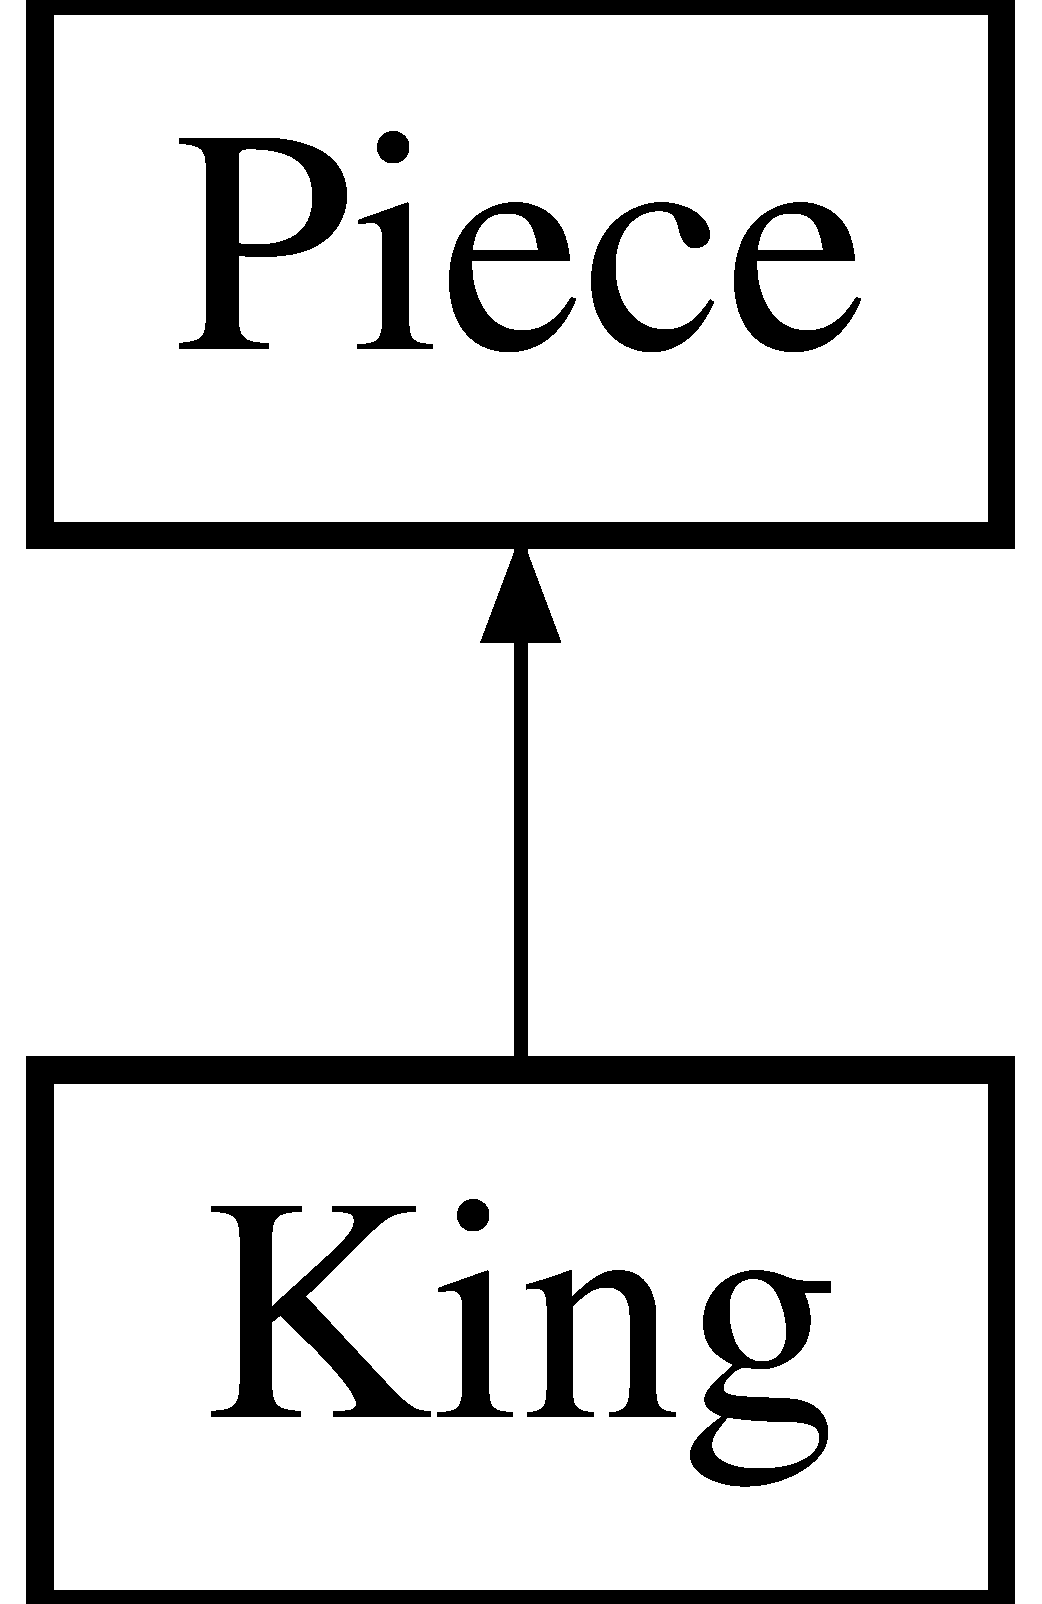
\includegraphics[height=2.000000cm]{class_king}
\end{center}
\end{figure}
\subsection*{Public Member Functions}
\begin{DoxyCompactItemize}
\item 
\hypertarget{class_king_a9b6b029c60a7b8a16f7221fbbf1285c9}{void {\bfseries update\-Moves} (\hyperlink{class_piece}{Piece}\mbox{[}$\,$\mbox{]}\mbox{[}$\,$\mbox{]} spaces, int rank, int file)}\label{class_king_a9b6b029c60a7b8a16f7221fbbf1285c9}

\end{DoxyCompactItemize}
\subsection*{Additional Inherited Members}


The documentation for this class was generated from the following file\-:\begin{DoxyCompactItemize}
\item 
src/King.\-java\end{DoxyCompactItemize}

\hypertarget{class_knight}{\section{Knight Class Reference}
\label{class_knight}\index{Knight@{Knight}}
}
Inheritance diagram for Knight\-:\begin{figure}[H]
\begin{center}
\leavevmode
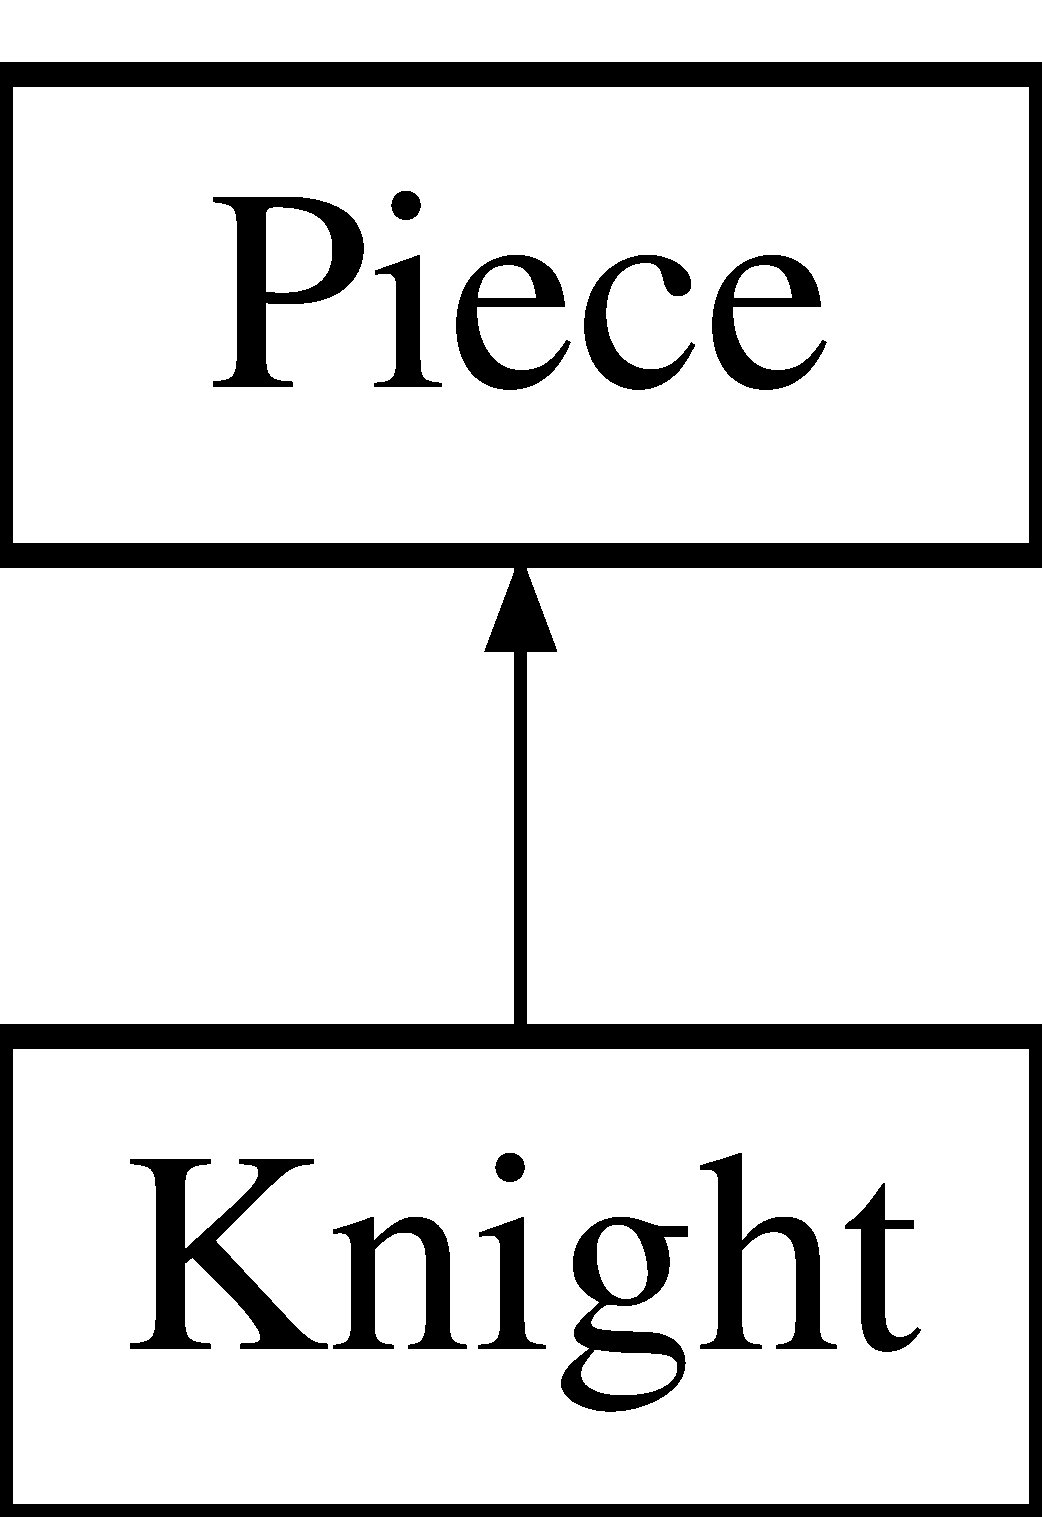
\includegraphics[height=2.000000cm]{class_knight}
\end{center}
\end{figure}
\subsection*{Public Member Functions}
\begin{DoxyCompactItemize}
\item 
void \hyperlink{class_knight_aaec127931cdd68af4c0169c4ce221cc3}{update\-Moves} (\hyperlink{class_piece}{Piece}\mbox{[}$\,$\mbox{]}\mbox{[}$\,$\mbox{]} spaces, int rank, int file)
\end{DoxyCompactItemize}
\subsection*{Additional Inherited Members}


\subsection{Detailed Description}
\begin{DoxyAuthor}{Author}
Will 
\end{DoxyAuthor}


\subsection{Member Function Documentation}
\hypertarget{class_knight_aaec127931cdd68af4c0169c4ce221cc3}{\index{Knight@{Knight}!update\-Moves@{update\-Moves}}
\index{update\-Moves@{update\-Moves}!Knight@{Knight}}
\subsubsection[{update\-Moves}]{\setlength{\rightskip}{0pt plus 5cm}void Knight.\-update\-Moves (
\begin{DoxyParamCaption}
\item[{{\bf Piece}}]{spaces\mbox{[}$\,$\mbox{]}\mbox{[}$\,$\mbox{]}, }
\item[{int}]{rank, }
\item[{int}]{file}
\end{DoxyParamCaption}
)}}\label{class_knight_aaec127931cdd68af4c0169c4ce221cc3}
Updates the possible moves for the piece. Knights can move in L-\/shapes (combinations of 2 in one direction and 1 in another). 
\begin{DoxyParams}{Parameters}
{\em spaces} & the current board state \\
\hline
{\em rank} & the x (rank) location of the piece \\
\hline
{\em file} & the y (file) location of the piece \\
\hline
\end{DoxyParams}


The documentation for this class was generated from the following file\-:\begin{DoxyCompactItemize}
\item 
src/Knight.\-java\end{DoxyCompactItemize}

\hypertarget{class_pawn}{\section{Pawn Class Reference}
\label{class_pawn}\index{Pawn@{Pawn}}
}
Inheritance diagram for Pawn\-:\begin{figure}[H]
\begin{center}
\leavevmode
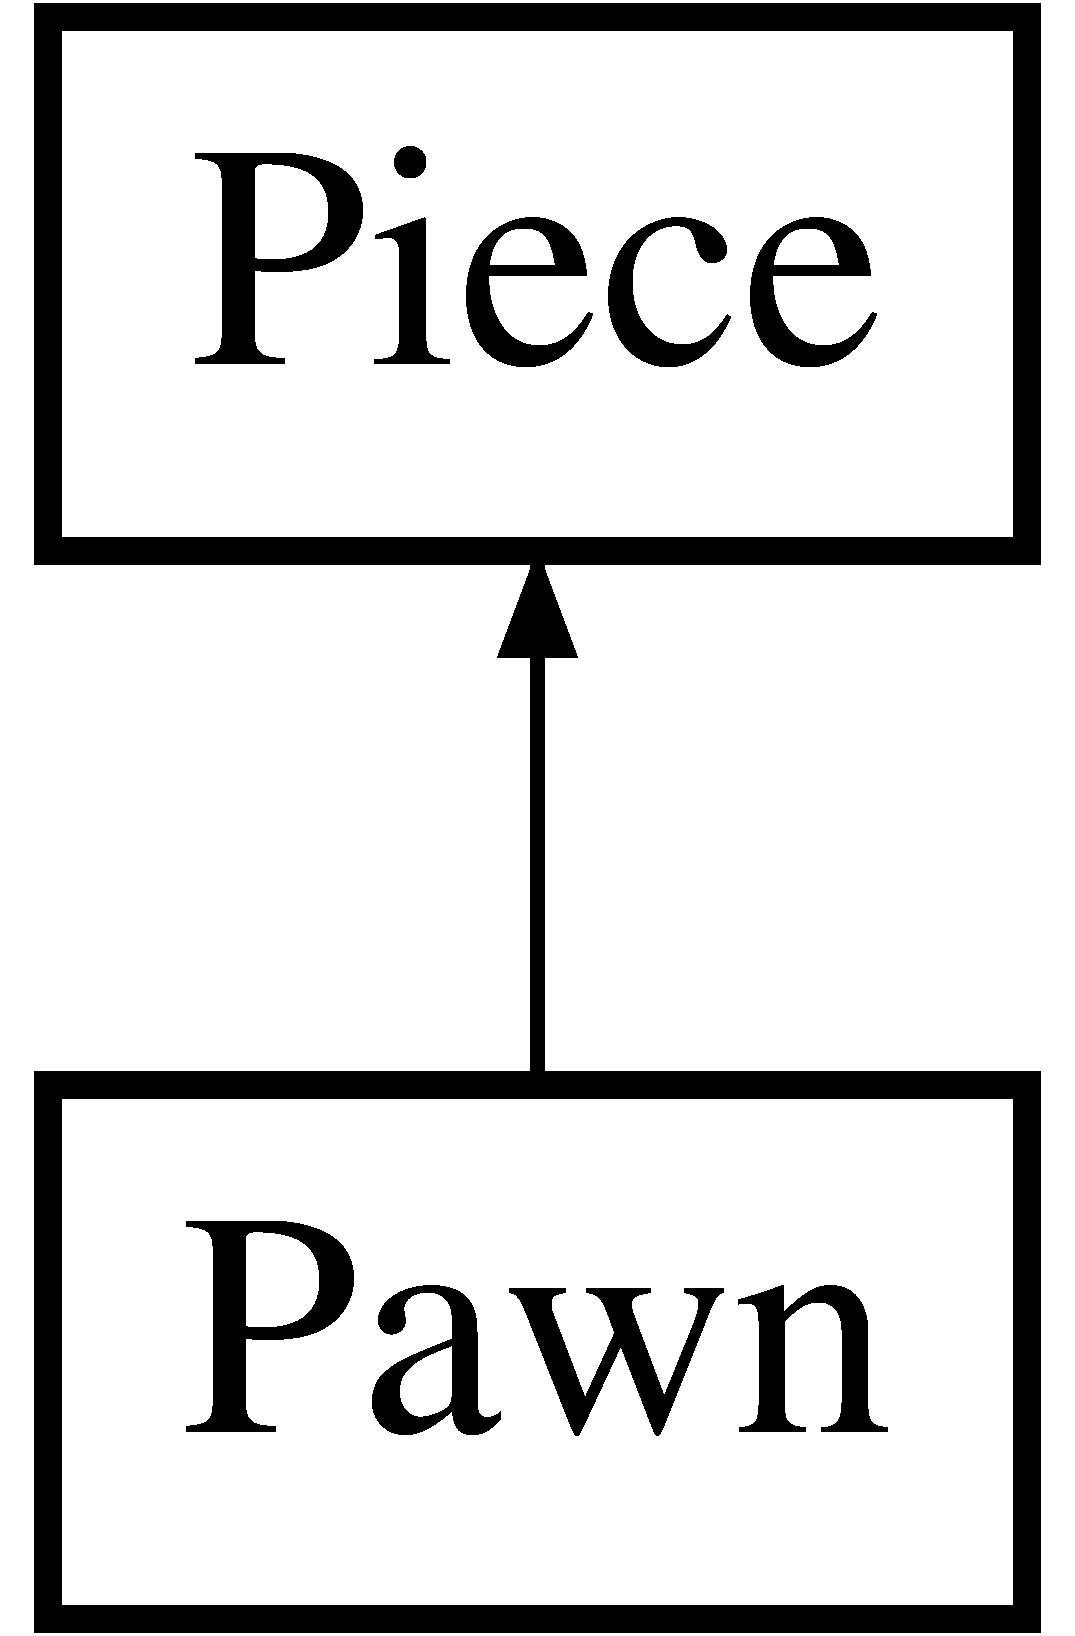
\includegraphics[height=2.000000cm]{class_pawn}
\end{center}
\end{figure}
\subsection*{Public Member Functions}
\begin{DoxyCompactItemize}
\item 
\hypertarget{class_pawn_aecc2590ecf87f465a7593ef67569fc47}{void {\bfseries update\-Moves} (\hyperlink{class_piece}{Piece}\mbox{[}$\,$\mbox{]}\mbox{[}$\,$\mbox{]} spaces, int rank, int file)}\label{class_pawn_aecc2590ecf87f465a7593ef67569fc47}

\end{DoxyCompactItemize}
\subsection*{Additional Inherited Members}


The documentation for this class was generated from the following file\-:\begin{DoxyCompactItemize}
\item 
src/Pawn.\-java\end{DoxyCompactItemize}

\hypertarget{class_piece}{\section{Piece Class Reference}
\label{class_piece}\index{Piece@{Piece}}
}
Inheritance diagram for Piece\-:\begin{figure}[H]
\begin{center}
\leavevmode
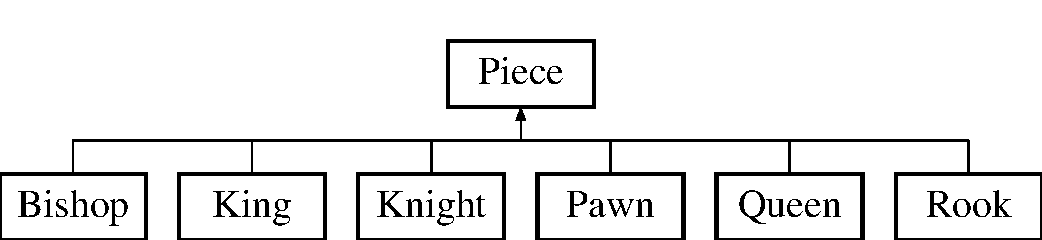
\includegraphics[height=2.000000cm]{class_piece}
\end{center}
\end{figure}
\subsection*{Public Member Functions}
\begin{DoxyCompactItemize}
\item 
abstract void \hyperlink{class_piece_a4a6c2b5c5d4dd5e3fa08f3a4cb97c9ba}{update\-Moves} (\hyperlink{class_piece}{Piece}\mbox{[}$\,$\mbox{]}\mbox{[}$\,$\mbox{]} spaces, int rank, int file)
\item 
boolean \hyperlink{class_piece_a6c777344ee49d908f6c3cf43948a204d}{is\-Valid\-Move} (\hyperlink{class_space}{Space} target)
\item 
Color \hyperlink{class_piece_a076592733b1498c5bc04ac61059eb1cc}{get\-Color} ()
\item 
boolean \hyperlink{class_piece_a3b293d270e867e61341b27df6d71c5da}{same\-Owner} (\hyperlink{class_piece}{Piece} other)
\end{DoxyCompactItemize}
\subsection*{Static Public Member Functions}
\begin{DoxyCompactItemize}
\item 
static \hyperlink{class_piece}{Piece} \hyperlink{class_piece_aa6ae6ab5e1f16bdb941f9798362b3c66}{string\-To\-Piece} (String piece, Color player)
\end{DoxyCompactItemize}
\subsection*{Protected Member Functions}
\begin{DoxyCompactItemize}
\item 
void \hyperlink{class_piece_aa9ea4ff0dd0e931fc3ad928233fbd281}{set\-Color} (Color player)
\item 
boolean \hyperlink{class_piece_a9dfc2ca9c8375ca29deb561255c4ce9b}{add\-Move} (\hyperlink{class_piece}{Piece} cur\-Space, int rank, int file)
\item 
boolean \hyperlink{class_piece_a140ea5008973d6cceb3ede41ef57b2c1}{out\-Of\-Bounds} (\hyperlink{class_piece}{Piece}\mbox{[}$\,$\mbox{]}\mbox{[}$\,$\mbox{]} spaces, int rank, int file)
\end{DoxyCompactItemize}
\subsection*{Protected Attributes}
\begin{DoxyCompactItemize}
\item 
\hypertarget{class_piece_ac3be06c38af4366f18cef94594a30a0d}{Color {\bfseries color} = null}\label{class_piece_ac3be06c38af4366f18cef94594a30a0d}

\item 
\hypertarget{class_piece_a6fb158d95f588f706ae716b13487ba10}{Vector$<$ \hyperlink{class_space}{Space} $>$ {\bfseries moves}}\label{class_piece_a6fb158d95f588f706ae716b13487ba10}

\end{DoxyCompactItemize}


\subsection{Member Function Documentation}
\hypertarget{class_piece_a9dfc2ca9c8375ca29deb561255c4ce9b}{\index{Piece@{Piece}!add\-Move@{add\-Move}}
\index{add\-Move@{add\-Move}!Piece@{Piece}}
\subsubsection[{add\-Move}]{\setlength{\rightskip}{0pt plus 5cm}boolean Piece.\-add\-Move (
\begin{DoxyParamCaption}
\item[{{\bf Piece}}]{cur\-Space, }
\item[{int}]{rank, }
\item[{int}]{file}
\end{DoxyParamCaption}
)\hspace{0.3cm}{\ttfamily [protected]}}}\label{class_piece_a9dfc2ca9c8375ca29deb561255c4ce9b}
Update\-Moves helper that checks if a given square should be added. \begin{DoxyReturn}{Returns}
true if the piece cannot jump past the square 
\end{DoxyReturn}
\hypertarget{class_piece_a076592733b1498c5bc04ac61059eb1cc}{\index{Piece@{Piece}!get\-Color@{get\-Color}}
\index{get\-Color@{get\-Color}!Piece@{Piece}}
\subsubsection[{get\-Color}]{\setlength{\rightskip}{0pt plus 5cm}Color Piece.\-get\-Color (
\begin{DoxyParamCaption}
{}
\end{DoxyParamCaption}
)}}\label{class_piece_a076592733b1498c5bc04ac61059eb1cc}
\begin{DoxyReturn}{Returns}
W\-H\-I\-T\-E,B\-L\-A\-C\-K,or N\-U\-L\-L 
\end{DoxyReturn}
\hypertarget{class_piece_a6c777344ee49d908f6c3cf43948a204d}{\index{Piece@{Piece}!is\-Valid\-Move@{is\-Valid\-Move}}
\index{is\-Valid\-Move@{is\-Valid\-Move}!Piece@{Piece}}
\subsubsection[{is\-Valid\-Move}]{\setlength{\rightskip}{0pt plus 5cm}boolean Piece.\-is\-Valid\-Move (
\begin{DoxyParamCaption}
\item[{{\bf Space}}]{target}
\end{DoxyParamCaption}
)}}\label{class_piece_a6c777344ee49d908f6c3cf43948a204d}

\begin{DoxyParams}{Parameters}
{\em target} & \\
\hline
\end{DoxyParams}
\begin{DoxyReturn}{Returns}

\end{DoxyReturn}
\hypertarget{class_piece_a140ea5008973d6cceb3ede41ef57b2c1}{\index{Piece@{Piece}!out\-Of\-Bounds@{out\-Of\-Bounds}}
\index{out\-Of\-Bounds@{out\-Of\-Bounds}!Piece@{Piece}}
\subsubsection[{out\-Of\-Bounds}]{\setlength{\rightskip}{0pt plus 5cm}boolean Piece.\-out\-Of\-Bounds (
\begin{DoxyParamCaption}
\item[{Piecespaces}]{\mbox{[}$\,$\mbox{]}\mbox{[}$\,$\mbox{]}, }
\item[{int}]{rank, }
\item[{int}]{file}
\end{DoxyParamCaption}
)\hspace{0.3cm}{\ttfamily [protected]}}}\label{class_piece_a140ea5008973d6cceb3ede41ef57b2c1}

\begin{DoxyParams}{Parameters}
{\em spaces} & \\
\hline
{\em rank} & \\
\hline
{\em file} & \\
\hline
\end{DoxyParams}
\begin{DoxyReturn}{Returns}

\end{DoxyReturn}
\hypertarget{class_piece_a3b293d270e867e61341b27df6d71c5da}{\index{Piece@{Piece}!same\-Owner@{same\-Owner}}
\index{same\-Owner@{same\-Owner}!Piece@{Piece}}
\subsubsection[{same\-Owner}]{\setlength{\rightskip}{0pt plus 5cm}boolean Piece.\-same\-Owner (
\begin{DoxyParamCaption}
\item[{{\bf Piece}}]{other}
\end{DoxyParamCaption}
)}}\label{class_piece_a3b293d270e867e61341b27df6d71c5da}

\begin{DoxyParams}{Parameters}
{\em other} & \\
\hline
\end{DoxyParams}
\begin{DoxyReturn}{Returns}

\end{DoxyReturn}
\hypertarget{class_piece_aa9ea4ff0dd0e931fc3ad928233fbd281}{\index{Piece@{Piece}!set\-Color@{set\-Color}}
\index{set\-Color@{set\-Color}!Piece@{Piece}}
\subsubsection[{set\-Color}]{\setlength{\rightskip}{0pt plus 5cm}void Piece.\-set\-Color (
\begin{DoxyParamCaption}
\item[{Color}]{player}
\end{DoxyParamCaption}
)\hspace{0.3cm}{\ttfamily [protected]}}}\label{class_piece_aa9ea4ff0dd0e931fc3ad928233fbd281}

\begin{DoxyParams}{Parameters}
{\em player} & \\
\hline
\end{DoxyParams}
\hypertarget{class_piece_aa6ae6ab5e1f16bdb941f9798362b3c66}{\index{Piece@{Piece}!string\-To\-Piece@{string\-To\-Piece}}
\index{string\-To\-Piece@{string\-To\-Piece}!Piece@{Piece}}
\subsubsection[{string\-To\-Piece}]{\setlength{\rightskip}{0pt plus 5cm}static {\bf Piece} Piece.\-string\-To\-Piece (
\begin{DoxyParamCaption}
\item[{String}]{piece, }
\item[{Color}]{player}
\end{DoxyParamCaption}
)\hspace{0.3cm}{\ttfamily [static]}}}\label{class_piece_aa6ae6ab5e1f16bdb941f9798362b3c66}

\begin{DoxyParams}{Parameters}
{\em piece} & \\
\hline
{\em player} & \\
\hline
\end{DoxyParams}
\begin{DoxyReturn}{Returns}

\end{DoxyReturn}
\hypertarget{class_piece_a4a6c2b5c5d4dd5e3fa08f3a4cb97c9ba}{\index{Piece@{Piece}!update\-Moves@{update\-Moves}}
\index{update\-Moves@{update\-Moves}!Piece@{Piece}}
\subsubsection[{update\-Moves}]{\setlength{\rightskip}{0pt plus 5cm}abstract void Piece.\-update\-Moves (
\begin{DoxyParamCaption}
\item[{{\bf Piece}}]{spaces\mbox{[}$\,$\mbox{]}\mbox{[}$\,$\mbox{]}, }
\item[{int}]{rank, }
\item[{int}]{file}
\end{DoxyParamCaption}
)\hspace{0.3cm}{\ttfamily [abstract]}}}\label{class_piece_a4a6c2b5c5d4dd5e3fa08f3a4cb97c9ba}

\begin{DoxyParams}{Parameters}
{\em spaces} & \\
\hline
{\em rank} & \\
\hline
{\em file} & \\
\hline
\end{DoxyParams}


The documentation for this class was generated from the following file\-:\begin{DoxyCompactItemize}
\item 
src/Piece.\-java\end{DoxyCompactItemize}

\hypertarget{class_queen}{\section{Queen Class Reference}
\label{class_queen}\index{Queen@{Queen}}
}
Inheritance diagram for Queen\-:\begin{figure}[H]
\begin{center}
\leavevmode
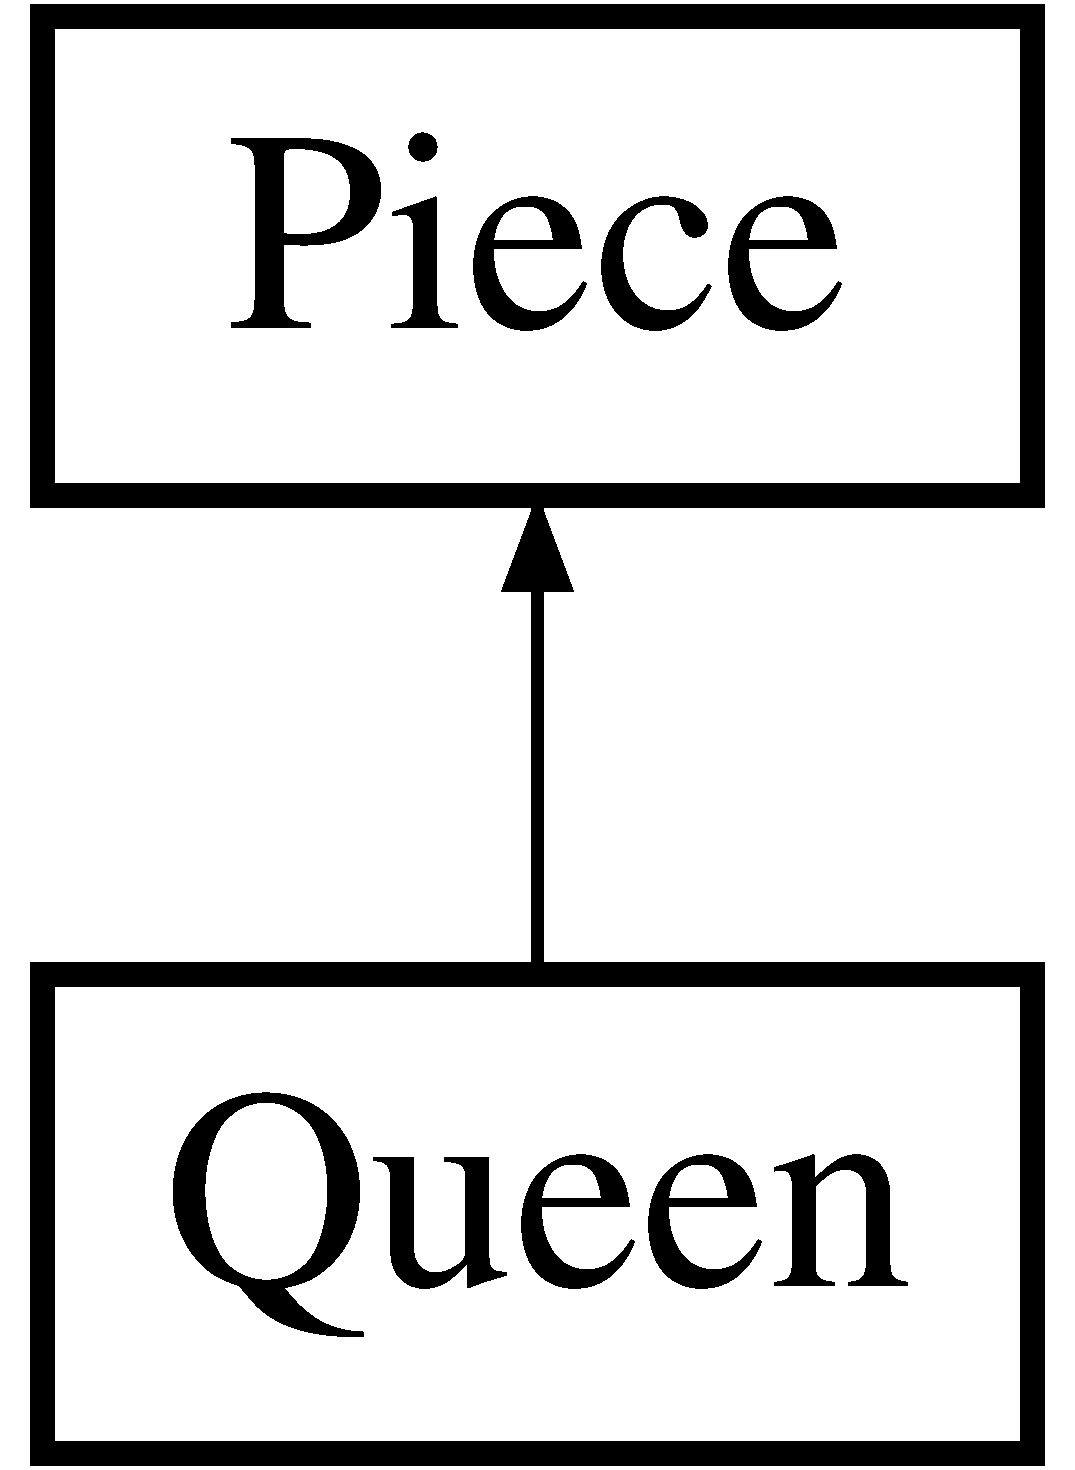
\includegraphics[height=2.000000cm]{class_queen}
\end{center}
\end{figure}
\subsection*{Public Member Functions}
\begin{DoxyCompactItemize}
\item 
void \hyperlink{class_queen_a680fb8dbed426be9577d3b63cabc2a53}{update\-Moves} (\hyperlink{class_piece}{Piece}\mbox{[}$\,$\mbox{]}\mbox{[}$\,$\mbox{]} spaces, int rank, int file)
\end{DoxyCompactItemize}
\subsection*{Additional Inherited Members}


\subsection{Detailed Description}
\begin{DoxyAuthor}{Author}
Will 
\end{DoxyAuthor}


\subsection{Member Function Documentation}
\hypertarget{class_queen_a680fb8dbed426be9577d3b63cabc2a53}{\index{Queen@{Queen}!update\-Moves@{update\-Moves}}
\index{update\-Moves@{update\-Moves}!Queen@{Queen}}
\subsubsection[{update\-Moves}]{\setlength{\rightskip}{0pt plus 5cm}void Queen.\-update\-Moves (
\begin{DoxyParamCaption}
\item[{{\bf Piece}}]{spaces\mbox{[}$\,$\mbox{]}\mbox{[}$\,$\mbox{]}, }
\item[{int}]{rank, }
\item[{int}]{file}
\end{DoxyParamCaption}
)}}\label{class_queen_a680fb8dbed426be9577d3b63cabc2a53}
Updates the possible moves for the piece. Queens can move as many squares as possible in any direction. 
\begin{DoxyParams}{Parameters}
{\em spaces} & the current board state \\
\hline
{\em rank} & the x (rank) location of the piece \\
\hline
{\em file} & the y (file) location of the piece \\
\hline
\end{DoxyParams}


The documentation for this class was generated from the following file\-:\begin{DoxyCompactItemize}
\item 
src/Queen.\-java\end{DoxyCompactItemize}

\hypertarget{class_rook}{\section{Rook Class Reference}
\label{class_rook}\index{Rook@{Rook}}
}
Inheritance diagram for Rook\-:\begin{figure}[H]
\begin{center}
\leavevmode
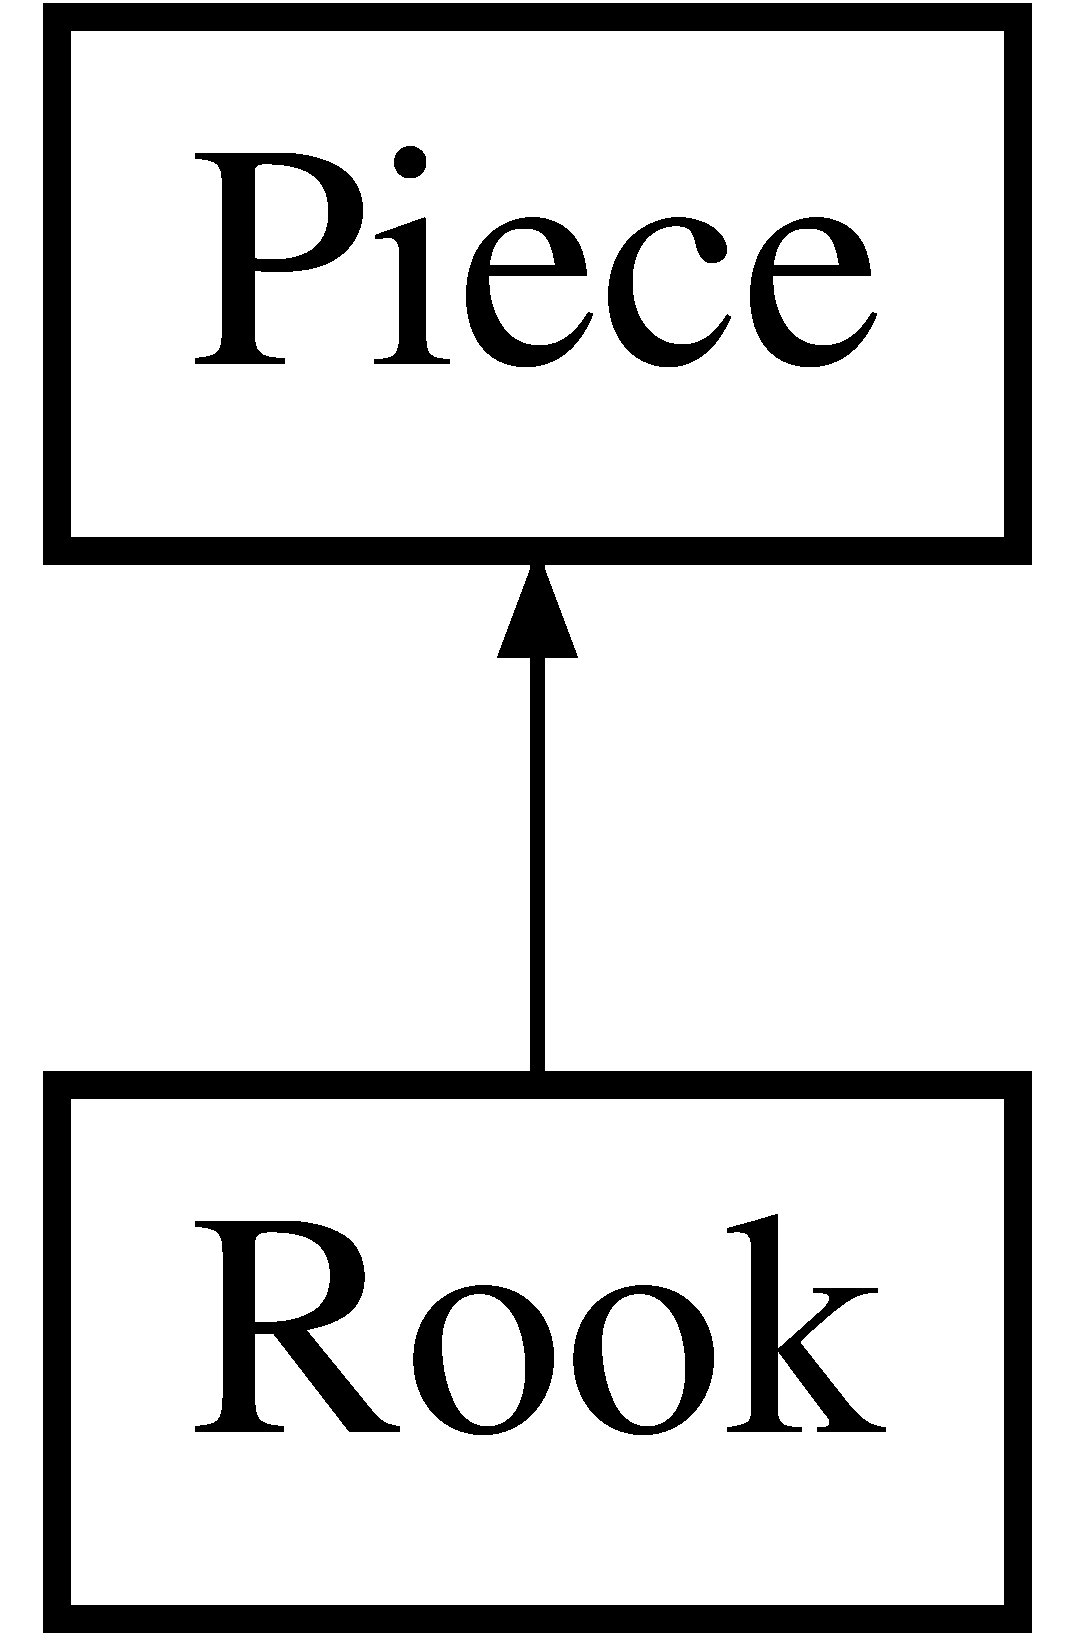
\includegraphics[height=2.000000cm]{class_rook}
\end{center}
\end{figure}
\subsection*{Public Member Functions}
\begin{DoxyCompactItemize}
\item 
void \hyperlink{class_rook_ac9bc900686605e24c20fc5d437331934}{update\-Moves} (\hyperlink{class_piece}{Piece}\mbox{[}$\,$\mbox{]}\mbox{[}$\,$\mbox{]} spaces, int rank, int file)
\end{DoxyCompactItemize}
\subsection*{Additional Inherited Members}


\subsection{Detailed Description}
\begin{DoxyAuthor}{Author}
Will 
\end{DoxyAuthor}


\subsection{Member Function Documentation}
\hypertarget{class_rook_ac9bc900686605e24c20fc5d437331934}{\index{Rook@{Rook}!update\-Moves@{update\-Moves}}
\index{update\-Moves@{update\-Moves}!Rook@{Rook}}
\subsubsection[{update\-Moves}]{\setlength{\rightskip}{0pt plus 5cm}void Rook.\-update\-Moves (
\begin{DoxyParamCaption}
\item[{Piecespaces}]{\mbox{[}$\,$\mbox{]}\mbox{[}$\,$\mbox{]}, }
\item[{int}]{rank, }
\item[{int}]{file}
\end{DoxyParamCaption}
)}}\label{class_rook_ac9bc900686605e24c20fc5d437331934}
Upates the possible moves for a given piece. Rooks can move in straight lines horizontal and vertical. 
\begin{DoxyParams}{Parameters}
{\em spaces} & the state of the chess board. \\
\hline
{\em rank} & the x (rank) location of the piece \\
\hline
{\em file} & the y (file) location of the piece \\
\hline
\end{DoxyParams}


The documentation for this class was generated from the following file\-:\begin{DoxyCompactItemize}
\item 
src/Rook.\-java\end{DoxyCompactItemize}

\hypertarget{class_space}{\section{Space Class Reference}
\label{class_space}\index{Space@{Space}}
}
\subsection*{Public Member Functions}
\begin{DoxyCompactItemize}
\item 
\hyperlink{class_space_a393206a3e5512fcba4d47c371897b971}{Space} (int r, int f)
\item 
int \hyperlink{class_space_a5091079d7ca873568f5591aaba39f4d1}{rank} ()
\item 
int \hyperlink{class_space_a3c4bed7fb0652ace48d61b074ffba54e}{file} ()
\item 
boolean \hyperlink{class_space_ac87fd1a8e63324c66114ea6bebd9a3b9}{equals} (\hyperlink{class_space}{Space} other)
\end{DoxyCompactItemize}


\subsection{Detailed Description}
\begin{DoxyAuthor}{Author}
Will 
\end{DoxyAuthor}


\subsection{Constructor \& Destructor Documentation}
\hypertarget{class_space_a393206a3e5512fcba4d47c371897b971}{\index{Space@{Space}!Space@{Space}}
\index{Space@{Space}!Space@{Space}}
\subsubsection[{Space}]{\setlength{\rightskip}{0pt plus 5cm}Space.\-Space (
\begin{DoxyParamCaption}
\item[{int}]{r, }
\item[{int}]{f}
\end{DoxyParamCaption}
)}}\label{class_space_a393206a3e5512fcba4d47c371897b971}

\begin{DoxyParams}{Parameters}
{\em r} & the rank (x position) of a board space \\
\hline
{\em f} & the file (y position) of a board space \\
\hline
\end{DoxyParams}


\subsection{Member Function Documentation}
\hypertarget{class_space_ac87fd1a8e63324c66114ea6bebd9a3b9}{\index{Space@{Space}!equals@{equals}}
\index{equals@{equals}!Space@{Space}}
\subsubsection[{equals}]{\setlength{\rightskip}{0pt plus 5cm}boolean Space.\-equals (
\begin{DoxyParamCaption}
\item[{{\bf Space}}]{other}
\end{DoxyParamCaption}
)}}\label{class_space_ac87fd1a8e63324c66114ea6bebd9a3b9}

\begin{DoxyParams}{Parameters}
{\em other} & the other space (rank,file) to compare to \\
\hline
\end{DoxyParams}
\begin{DoxyReturn}{Returns}
true if one space the same (x,y) position of another 
\end{DoxyReturn}
\hypertarget{class_space_a3c4bed7fb0652ace48d61b074ffba54e}{\index{Space@{Space}!file@{file}}
\index{file@{file}!Space@{Space}}
\subsubsection[{file}]{\setlength{\rightskip}{0pt plus 5cm}int Space.\-file (
\begin{DoxyParamCaption}
{}
\end{DoxyParamCaption}
)}}\label{class_space_a3c4bed7fb0652ace48d61b074ffba54e}
\begin{DoxyReturn}{Returns}
the file (y position) of a given space 
\end{DoxyReturn}
\hypertarget{class_space_a5091079d7ca873568f5591aaba39f4d1}{\index{Space@{Space}!rank@{rank}}
\index{rank@{rank}!Space@{Space}}
\subsubsection[{rank}]{\setlength{\rightskip}{0pt plus 5cm}int Space.\-rank (
\begin{DoxyParamCaption}
{}
\end{DoxyParamCaption}
)}}\label{class_space_a5091079d7ca873568f5591aaba39f4d1}
\begin{DoxyReturn}{Returns}
the rank (x position) of a given space 
\end{DoxyReturn}


The documentation for this class was generated from the following file\-:\begin{DoxyCompactItemize}
\item 
src/Space.\-java\end{DoxyCompactItemize}

%--- End generated contents ---

% Index
\newpage
\phantomsection
\addcontentsline{toc}{chapter}{Index}
\printindex

\end{document}
